\documentclass{article}
\usepackage[table,xcdraw]{xcolor}
\usepackage[utf8]{inputenc}
\usepackage{geometry}
\usepackage{amsmath}
\usepackage{amsthm}
\usepackage{amsfonts}
\usepackage{amssymb}
\usepackage{graphicx}
\usepackage{tocloft}
\usepackage{pgfplots}
\usepackage{multirow}	

\usepackage[usenames,dvipsnames]{pstricks}
\usepackage{epsfig}
\usepackage{pst-grad} % For gradients
\usepackage{pst-plot} % For axes
\usepackage[space]{grffile} % For spaces in paths
\usepackage{etoolbox} % For spaces in paths

%\usepackage{perpage} %the perpage package
%\MakePerPage{footnote} %the perpage package command

% For adding TOC in pdf bookmarks
\usepackage{hyperref}
\hypersetup{pdftex,colorlinks=true,allcolors=black}
\usepackage{hypcap}
%
\usepackage{float}
\usepackage{listings}
\usepackage{color}

\definecolor{codegreen}{rgb}{0,0.6,0}
\definecolor{codegray}{rgb}{0.5,0.5,0.5}
\definecolor{codepurple}{rgb}{0.58,0,0.82}
\definecolor{backcolour}{rgb}{0.95,0.95,0.92}

\lstdefinestyle{mystyle}{
	backgroundcolor=\color{backcolour},   
	commentstyle=\color{codegreen},
	keywordstyle=\color{magenta},
	numberstyle=\tiny\color{codegray},
	stringstyle=\color{codepurple},
	basicstyle=\footnotesize,
	breakatwhitespace=false,         
	breaklines=true,                 
	captionpos=b,                    
	keepspaces=true,                 
	numbers=left,                    
	numbersep=5pt,                  
	showspaces=false,                
	showstringspaces=false,
	showtabs=false,                  
	tabsize=2
}

\lstset{style=mystyle}
\usepackage{xepersian}
\usepackage{bidi}

\settextfont{Yas}
\SepMark{-}

\renewcommand{\cftsecleader}{\cftdotfill{\cftdotsep}}

\theoremstyle{definition}
\newtheorem{definition}{تعریف}

\providecommand{\keywords}[1]{
	\vspace{1cm}
	\textbf{
		\textit{
			کلمات کلیدی:
			}
		} #1
	}

\title{گزارش پروژه اول درس هوش مصنوعی و سیستم‌های خبره}
\author{امیر حقیقتی ملکی}
\date{بهار ۹۶}
	
\begin{document}
	%%%%%%%%%%%%%%%%%%%%%%%%%%%%%%%
	%%	 TITLE PAGE - BEGIN	     %%
	%%%%%%%%%%%%%%%%%%%%%%%%%%%%%%%
	\newgeometry{margin=1in}
	\pagenumbering{gobble}
		\begin{titlepage}
		\centering
		
\includegraphics[width=0.35\textwidth]{Resources/logo.png}\par\vspace{1cm}
		{\scshape\LARGE دانشگاه صنعتی امیرکبیر \par}
		{\scshape\LARGE دانشکده مهندسی کامپیوتر و فناوری اطلاعات \par}
		\vspace{1cm}
		{\scshape\Large
			گزارش پروژه اول درس
			«هوش مصنوعی و سیستم‌های خبره»
			\par}
		\vspace{1.5cm}
		{\huge\bfseries 
	حل مسئله با جستجو
			\par}
		\vspace{2cm}
		{\Large امیر حقیقتی ملکی\par}
		\vfill
		استاد:\par
		دکتر نیک‌آبادی
		\vfill
		
		% Bottom of the page
		{\large \rl{بهار ۹۶}\par}
	\end{titlepage}
	%%%%%%%%%%%%%%%%%%%%%%%%%%%%%%%
	%%	 ABSTRACT - BEGIN	     %%
	%%%%%%%%%%%%%%%%%%%%%%%%%%%%%%%
	\newpage
	%\restoregeometry
	\pagenumbering{Alph}
		\begin{abstract}
	حل مسئله با جستجوی درخت و در حالت کلی گراف فضای حالت مسئله یکی از روش‌های کلاسیک برای حل مسائلی است که در آن محیط کاملا قابل مشاهده، گسسته، شناخته شده و قطعی می‌باشد. در این روش، عامل‌های مبتنی بر هدف توصیف می‌شوند و با دادن فرموله‌بندی مناسبی از مسئله مورد نظر، می‌توان به راه‌حل (در صورت وجود) دست یافت. طبق تعریف پروژه، فریم‌ورکی\footnote{framework} برای این منظور پیاده‌سازی شد که در آن از الگوریتم‌های جستجوی گرافی اول سطح، اول عمق (عمق نامحدود، عمق محدود، افزایش تدریجی عمق)، هزینه یکنواخت، دو جهته که از جزو الگوریتم‌های جستجوی ناآگاهانه به حساب آمده و A* که یک الگوریتم جستجوی آگاهانه است، استفاده شد. این فریم‌ورک به زبان Java بوده و مستندات مربوط به استفاده از آن و نحوه فرموله‌بندی مسئله در این گزارش ذکر شده است. سه مسئله نمونه مسیریابی، پازل لغزشی و مبلغان مذهبی و آدم‌خوار‌ها در تعریف پروژه ذکر شده‌اند که با انجام فرموله‌بندی و انجام آزمایشات، پاسخ این مسائل و نتایج عملکرد هرکدام از الگوریتم‌های پیاده‌سازی شده مشخص شدند. الگوریتم جستجوی گرافی اول بهترین حریصانه نیز می‌تواند در آینده به منظور افزودن قابلیت‌های بیشتر به این فریم‌ورک اضافه شود.
	\end{abstract}
	\keywords{
		هوش مصنوعی، مسائل کلاسیک، حل مسئله با جستجو، جستجوی آگاهانه، جستجوی ناآگاهانه،
		جستجوی گراف
	}	
	%%%%%%%%%%%%%%%%%%%%%%%%%%%%%%%
	%%	TABLE OF CONTENTS		 %%
	%%%%%%%%%%%%%%%%%%%%%%%%%%%%%%%
	\newpage
	\pagenumbering{gobble}
	\tableofcontents
	%%%%%%%%%%%%%%%%%%%%%%%%%%%%%%%
	%%	   INTRODUCTION    		 %%
	%%%%%%%%%%%%%%%%%%%%%%%%%%%%%%%
	\newpage
	\pagenumbering{arabic}
	\section{مقدمه}
	عامل‌های هوشمند واکنشی ساده، در محیط‌هایی که تعداد حالات آن زیاد است و در مسائلی که به مسائل جهان واقعی نزدیک است نمی‌توانند بازدهی مناسبی داشته باشند و در نتیجه دیگر سادگی آن‌ها کارآمد نخواهد بود. برای حل مسائل واقعی، می‌توانیم از عامل‌های مبتنی بر هدفی که اعمال و اقدامات خود را پیش از انجام مورد سنجش قرار می‌دهند استفاده کنیم. این عامل‌ها، حالت‌های محیط خود را به دید اتمیک نگاه می‌کنند؛ به این معنی که در هر حالت، حالت فعلی دیگر قابل تقسیم به جزء های کوچک‌تر نیست. در این‌جا به منظور سادگی فرض می‌شود که راه‌حل یک مسئله، همواره دنباله‌ای ثابت از عملیات مختلف است؛ عمل‌های عامل در طول جستجو برای جواب، در اثر ورود ادراکات مختلف عوض نخواهند شد. با این مفروضات، روش‌ها و الگوریتم‌هایی که برای جستجوی راه‌حل در مسائلی از این قبیل در نظر گرفته می‌شوند می‌توانند از نوع آگاهانه یا ناآگاهانه باشند که در ادامه به توضیح آن‌ها پرداخته شده است.
	\subsection{عامل و محیط}
	عامل‌‌ها می‌توانند با دریافت ادراکات از محیط، با انجام عمل‌هایی روی محیط تاثیر گذاشته و حالت آن‌را عوض کنند و یا اینکه حالت کنونی خود در مقایسه با محیط را تغییر دهند. طبق تعریف عامل‌های هوشمند، می‌بایست فعالیت‌های این عامل‌ها منجر به بیشینه شدن معیار کارآیی\footnote{Performance measure} آن‌ها شود. گاهی اوقات، عامل می‌تواند با داشتن هدفی برای خود و تلاش برای رسیدن به آن هدف، معیار کارآیی خود را آسان‌تر به میزان بیشینه برساند. اهداف می‌توانند با محدود مقاصد عامل از انجام عمل‌های مختلف، در سامان‌دهی رفتار عامل کمک به سزایی داشته باشند. در نتیجه فرموله‌کردن هدف و مقصد مورد نظر - براساس موقعیت و حالت کنونی عامل و معیار کارآیی آن - اولین قدم برای حل مسئله می‌باشد.\\
	\paragraph{هدف}
	برای ما، مجموعه‌ای از چند حالت محیط می‌باشد که عامل می‌تواند با انجام عمل‌های مختلف خود را در آن حالت(ها) قرار دهد و به مقصود خود دست یابد؛ برای این منظور عامل می‌بایست مشخص کند که چه عملیاتی باید انجام دهد.\\
	پیش از تصمیم درباره عمل خاصی، عامل باید بداند که باید چه نوع عمل‌هایی را برای انجام و چه حالت‌هایی از محیط را برای رسیدن باید در نظر بگیرد. فرموله‌کردن مسئله به معنی تعریف و توصیف دقیق حالت‌ها و عملیات ممکن با توجه به حالت‌های هدف در یک محیط است. سطح تجرید عملیات‌ها و همچنین میزان جزئیات توصیف حالت‌های محیط می‌تواند بسته به مسئله متفاوت باشد و باید حتما به این نکته توجه شود که ذکر جزئیات بیش از حد و یا کم‌تر از میزان قابل قبول می‌تواند به عدم موفقیت عامل در دستیابی به پاسخ و رسیدن به هدف شود.
	\paragraph{محیط}
	برای تصمیم‌گیری در مورد انجام عملیات مختلف، عامل می‌بایست ابتدا بداند که در حالت کنونی خود مجاز به انجام چه عملیاتی است و نتیجه هر عمل منجر به رسیدن به کدام حالت از محیط می‌شود؛ سپس با بررسی هر عمل و با در نظر داشتن هدف، می‌تواند بهترین تصمیم را بگیرد. بنابراین فرض می‌شود که محیط
	\textbf{کاملا قابل مشاهده}
	است. همچنین در صورت نامحدود بودن عملیات قابل انجام در هر حالت، امکان تصمیم‌گیری برای عامل در عمل وجود نخواهد داشت. در نتیجه محیط می‌بایست
	\textbf{گسسته}
	باشد. به این معنی که در هر حالت، تعداد محدودی عمل قابل انجام است. همچنین در فرآیند تصمیم‌گیری، عامل مورد نظر ما می‌بایست قادر به پیش‌بینی نتیجه حاصل از عمل خود باشد. در غیر این‌صورت قادر به تصمیم‌گیری نخواهد بود. به عبارت دیگر فرض می‌شود محیط
	\textbf{شناخته شده}
	است و عامل می‌داند که با انجام هر عمل از حالت فعلی به کدام حالت می‌تواند برود. همچنین عدم قطعیت اعمال به کلی نادیده گرفته می‌شود و هر عامل در صورت انجام عملی، حتما و الزاما خروجی مربوط به آن عمل را خواهد دید. بنابراین محیط
	\textbf{قطعی}
	است.
	\paragraph{جستجو}
	فرآیند یافتن دنباله‌ای از عملیات که منجر به رسیدن به هدف شود جستجوی راه‌حل نام دارد. یک الگوریتم جستجوی راه‌حل، مسئله‌ای (فضای حالت)‌ را به عنوان ورودی گرفته و راه‌حل آن مسئله را در قالب دنباله‌ای از عملیات و اقدامات توصیف کرده و برمی‌گرداند.الگوریتم‌های مختلفی برای جستجوی راه‌حل در محیط‌های گوناگون وجود دارد که در ادامه به توضیح آن‌ها می‌پردازیم.\\
	هنگامی که راه‌حلی پیدا شد، می‌توان دنباله عملیات ذکر شده در راه‌حل را انجام داد؛ به این مرحله، مرحله اجرا گفته می‌شود. بنابراین برای رسیدن به هدف، می‌بایست ابتدا فرموله‌بندی مناسبی از مسائل و محیط ارائه دهیم، سپس راه‌حل را جستجو کنیم و در مرحله آخر، راه‌حل به دست آمده را برای اجرا به عامل بدهیم.\\
	\subsection{ساختار مسائل و راه‌حل‌ها}
	همانطور که در قسمت قبل ذکر شد، به دلیل گرافی بودن فضای حالت مسئله، برای فرموله کردن هر مسئله، گره‌های گراف را در قالب داده‌ساختاری به نام گره ذخیره می‌کنیم که این داده‌ساختار دارای مشخصه‌های زیر است:
	\begin{enumerate}
		\item
		آدرس گره پدر:
		برای یافتن مسیری که منتهی به این گره شده می‌بایست آدرس گره پدر را در هر گره ذخیره کنیم. این مشخصه در یافتن دنباله حالت‌های جستجو شده در راه‌حل مناسب می‌باشد.
		\item
		حالت عامل:
		حالتی که عامل با رسیدن به گره فعلی در آن قرار می‌گیرد در این داده‌ساختار ذخیره می‌شود.
		\item
		عمل انجام شده:
		عملی که با انجام آن به گره فعلی رسیده‌ایم و گره فعلی در نتیجه انجام آن عمل در حالت گره پدر می‌باشد. این مشخصه برای به دست آوردن دنباله عملیات انجام شده در طی یک راه‌حل مناسب می‌باشد.
		\item
		هزینه مسیر تا این گره:
		هزینه‌ای که تا این رسیدن به این گره پرداخت شده است. این مولفه برای به دست آوردن هزینه مسیر راه‌حل مناسب است.
	\end{enumerate}
	 همچنین به دلیل گرافی بودن فضای حالت مسئله، می‌بایست برای هر مسئله موارد زیر را تعریف کنیم:
	\begin{enumerate}
		\item
		ساختار کلی حالت‌ها:
		اینکه حالت‌ها در قالب ماتریس، عدد، رشته و یا غیره بیان می‌شوند، می‌بایست توسط مسئله بیان شود.
		\item
		حالت اولیه:
		حالت اولیه در واقع نشان دهنده پیکربندی\footnote{configuration} اولیه و حالت شروع عامل می‌باشد. این حالت در جستجوی راه‌حل به عنوان گره آغازین در نظر گرفته می‌شود و در راه‌حل پیدا شده نیز اولین گام خواهد بود.
		\item
		حالت هدف:
		درواقع اینکه عامل در مورد مسئله مورد نظر به حالت درستی رسیده یا نه توسط این حالت مشخص می‌شود. مقصد نهایی عامل می‌بایست اینجا باشد. در مسائلی که نتوان حالت هدف را به طور دقیق بیان کرد می‌بایست شرایط حالت هدف ذکر شود.
		\item
		نتیجه هر عمل در حالت‌های مختلف:
		از آن‌جا که فرض کرده‌ایم که محیط ما کاملا قابل مشاهده است، مسئله باید گویای نتیجه هر عمل (حالت حاصل شده در ازای انجام عمل) در هر حالتی از فضای حالت مسئله باشد.
		\item
		عملیات ممکن در هر حالت:
		پیرو مورد قبلی، از آن‌جا که فرض کرده‌ایم که محیط ما کاملا قابل مشاهده است، مسئله باید گویای عملیات قابل انجام توسط عامل در هر حالتی از فضای حالت باشد.
		\item
		هزینه انجام هر عمل در هر حالت:
		عامل باید بداند که هزینه انجام هر عمل در هر حالتی که باشد چقدر خواهد بود.
		\item
		هزینه مسیری که تا کنون پرداخت شده:
		عامل باید بداند که تا کنون و تا رسیدن به حالت فعلی چه هزینه‌ای پرداخت کرده است.
		\item
		تابع شهودی هزینه:
		این تابع که در واقع تخمینی است از هزینه باقی‌مانده تا رسیدن به حالت هدف، در صورتی باید پیاده‌سازی شود که بخواهیم از روش‌های جستجوهای آگاهانه در یافتن پاسخ استفاده کنیم.
	\end{enumerate}
در هر پیمایش و جستجوی راه‌حل، گرهیی ساخته می‌شود که پدر آن گره فعلی بوده و تمامی خصوصیت‌های نام برده شده نیز برای آن ست می‌شوند. اگر در حین جستجوی راه‌حل به گرهی برسیم که رمقصد مورد نظر عامل باشد، برای به دست آوردن دنباله اعمال انجام شده از حالت اولیه، کافی است از گره انتهایی (مقصد) که در جستجوی راه‌حل ساخته شده، شروع کرده و تا زمانی که به گره مبدا نرسیده‌ایم دنباله اعمال و حالت‌ها را بسازیم.
	
	
	
	
	

	
	
	
	
	
	
	
	
	%%%%%%%%%%%%%%%%%%%%%%%%%%%%%%%
	%%   METHODS AND MATERIALS   %%
	%%%%%%%%%%%%%%%%%%%%%%%%%%%%%%%
	\newpage
		\section{نحوه پیاده‌سازی، روش‌ها و الگوریتم‌ها}
	فریم‌ورک پیاده‌سازی شده توسط نگارنده به زبان Java بوده و
	\lr{GS-ProblemSolver}
	نام دارد که از چهار بسته\footnote{Package} به شرح زیر تشکیل شده است:
	\begin{itemize}
		\item
		بسته 
		\texttt{resources}:
		در این بسته، کلاس‌هایی که به طور مستقیم با پیمایش گراف و ساخته شدن راه‌حل در ارتباط هستند قرار دارند.
		\item
		بسته 
		\texttt{searchers}:
		هر جستجوگر که با الگوریتمی منحصر به فرد شروع به جستجو در فضای حالت مسئله می‌کند، در این بسته قرار داده شده است. این بسته حاوی کلاسی تحت عنوان
		\texttt{Searcher}
		است که به صورت ابسترکت\footnote{Abstract} پیاده‌سازی شده است. برای ثابت نگه داشتن واسط میان جستجوگرها و فضای حالت مسئله و همچنین واسط برنامه‌نویسی کاربری\footnote{API} کلاس‌های جستجوکننده، تمامی جستجوگرها می‌بایست از کلاس
		\texttt{Searcher}
		به ارث برده شوند\footnote{Inherit}.
		\item
		بسته
		\texttt{utilities}:
		شامل کلاس‌های کمکی در کار با فریم‌ورک است. در زمان ویراستاری این گزارش، در این بسته تنها کلاس
		\texttt{GSException}
		موجود است. این بسته بیشتر برای استفاده در آینده و افزودن کلاس‌های کمکی بیشتر به کار برده می‌شود. به عنوان مثال می‌توان در آینده کلاسی تحت عنوان تحلیل‌گر عملکرد جستجوگرها ساخت و در این بسته قرار داد.
		\item
		بسته 
		\texttt{main}:
		که حاوی برنامه اصلی و شروع‌کننده است.
	\end{itemize}
	توضیحات کلاس‌های موجود در هر بسته و نحوه پیاده‌سازی آن‌ها در ادامه ذکر می‌شود. شایان ذکر است تمامی توضیحات به صورت کامنت در کد منبع این پروژه نیز قرار دارند و توضیحات ذیل برای شفاف‌سازی بیشتر است.
	\subsection{کلاس‌های اصلی و منبع}
	همانطور که گفته شد، این کلاس‌ها به‌طور مستقیم با پیمایش فضای حالت مسئله و ساخته‌شدن راه‌حل ارتباط دارند. همگی این کلاس‌ها در بسته
	\texttt{resources}
	قرار گرفته‌اند و احتمال دارد که با ورود به فصل‌های بعدی کتاب و گسترش یافتن انواع مسئله‌ها و پیچیده‌تر شدن ساختار راه‌حل و نحوه جستجو، ساختار بعضی از کلاس‌ها تغییر یابد.
	\subsubsection{کلاس مسئله}
	این کلاس در فایل
	\texttt{Problem.java}
	 به صورت ابسترکت پیاده‌سازی شده و تنها دارای یک متد غیرابسترکت است. توابع این کلاس عبارتند از:
	\paragraph{تابع حالت اولیه}
	که در واقع تولیدکننده حالت ابتدایی و آغازین مسئله است. این تابع همچنین به ساختار حالت‌های مسئله قالب نیز می‌دهد و نوع‌داده آن‌ها را مشخص می‌کند.
	\begin{latin}
		\begin{lstlisting}[language=Java]
/**
* Getting the problem's initial state in which we start the search.
*
* @return State the initial state.
*/
public abstract State initialState();
\end{lstlisting}
	\end{latin}
	\paragraph{تابع تست هدف}
	این تابع برای بررسی اینکه آیا حالت داده شده هدف است یا نه مورد استفاده قرار می‌گیرد.
		\begin{latin}
		\begin{lstlisting}[language=Java]
/**
* Determine whether the given state is the goal of the problem or not.
*
* @param n State to review.
* @return boolean the answer.
*/
public abstract boolean goalTest(State n);
\end{lstlisting}
	\end{latin}
	\paragraph{تابع عمل‌های ممکن در هر حالت}
	عملیات ممکن در هر حالت توسط این تابع معلوم شده و برگردانده می‌شود. در این‌جا تمامی اعمال در نتیجه ظاهر نمی‌شوند و فقط اعمالی که قابلیت اجرا در حالت ورودی را دارند در نتیجه برگردانده می‌شوند.
		\begin{latin}
	\begin{lstlisting}[language=Java]
/**
* The actions list which can be performed while the agent is in state s.
*
* @param s State to review.
* @return Vector set of actions available in state s.
*/
public abstract Vector<Action> actions(State s);
\end{lstlisting}
	\end{latin}

	\paragraph{تابع معلوم‌کننده نتیجه هر عمل در یک حالت}
	به‌ازای عمل ورودی و قابل انجام در حالت ورودی، حالت نتیجه شدهدر صورت انجام آن عمل در حالت ورودی برگردانده می‌شود.
	\begin{latin}
		\begin{lstlisting}[language=Java]
/**
* Returns the result node of an action performed on agent when it was in state s.
*
* @param s State the state in which the agent is.
* @param a Action the action to perform.
* @return State with parent n.
*/
public abstract State result(State s, Action a);
\end{lstlisting}
	\end{latin}
	
	\paragraph{تابع هزینه عمل}
	هزینه انجام یک عمل در حالت ورودی را برمی‌گرداند. فرض براین است که عمل ورودی در حالت ذکر شده قابل انجام است.
	\begin{latin}
		\begin{lstlisting}[language=Java]
/**
* Returns the cost of action a in state s.
*
* @param s State in which the action will be performed.
* @param a Action to be performed
* @return double cost of the action.
*/
public abstract double actionCost(State s, Action a);
\end{lstlisting}
	\end{latin}

	\paragraph{تابع هزینه مسیر}
	هزینه مسیری که از حالت اولیه تا گره فعلی (دربردارنده حالت فعلی) طی شده را برمی‌گرداند.
		\begin{latin}
		\begin{lstlisting}[language=Java]
/**
* Returns the path in leaded to node n.
* @param n Node the leaf node.
* @return double path from root to leaf node n.
*/
public abstract double pathCost(Node n);
\end{lstlisting}
	\end{latin}

	\paragraph{تابع شهودی}
	فقط باید در صورتی پیاده‌سازی شود که از جستجوگرهای آگاهانه می‌خواهیم استفاده کنیم و در واقع این تابع مقدار
	\texttt{gScroe}
	را برای هر حالت تخمین می‌زند.
	\begin{latin}
		\begin{lstlisting}[language=Java]
/**
* Calculate the heuristic value for state s.
*
* @param s {@link State} the state to evaluate.
* @return int heuristic value.
*/
public abstract double heuristic(State s);
\end{lstlisting}
	\end{latin}

	\paragraph{تابع بازگرداننده راه‌حل}
	این تابع به صورت غیر ابسترکت پیاده‌سازی شده و به ازای هر ورودی که از جنس یک گره می‌باشد، حالت‌هایی که در هنگام جستجوی راه‌حل به‌دست آمده بودند را برمی‌گرداند. این تابع صرفا یک تابع کمکی است که به دست آوردن راه‌حل یک لایه تجرید بیشتر داشته باشد و آسان‌تر باشد. از ذکر جزئیات پیاده‌سازی این تابع پرهیز می‌شود؛ در صورت داشتن ابهام به کد منبع پروژه رجوع شود.
	
	\subsubsection{کلاس گره}
	این کلاس در فایل
	\texttt{Node.java}
	پیاده‌سازی شده و وظیفه نگهداری اطلاعات مربوط به مسیری که تا حالت کنونی طی شده است را دارد. شرط مساوی بودن یک گره با گره دیگر نیز مساوی بودن حالت‌های این دو گره است. در برخی جستجوها علاوه بر خصوصیات ذکر شده در قسمت‌های قبل، نیازمند دانستن عمق گره کنونی در گراف نیز هستیم که این خصوصیت از بررسی تعداد گره‌های موجود در مسیر منتهی به این گره به آسانی قابل حصول است و در داخل این کلاس نیز به عنوان یک تابع پیاده‌سازی شده است.
	\subsubsection{کلاس حالت}
	که در فایل
	\texttt{State.java}
	پیاده‌سازی شده است، دارای یک آبجکت\footnote{Object} به نام وضعیت\footnote{Status} و فقط به خاطر ساختارمند کردن هرچه بیشتر به عنوان یک کلاس پیاده‌سازی شده است. خصیصه وضعیت همان حالت مورد نظر است که به صورت اتمیک است.
	\subsubsection{کلاس عمل}
	این کلاس نیز در فایل
	\texttt{Action.java}
	پیاده‌سازی شده و تنها دارای دو خصیصه
	\texttt{data}
	و
	\texttt{cost}
	می‌باشد که اولی توضیحات و داده‌های مربوط به عمل است و دومی هزینه انجام عمل می‌باشد. همانند کلاس حالت، این کلاس نیز صرفا برای ساختارمند کردن بیشتر پروژه، پیاده‌سازی شده است.
	\subsection{جستجوگرها}
	این کلاس‌ها در بسته
	\texttt{searchers}
	قرار داشته و وظیفه یافتن راه‌حل برای مسئله پاس داده شده به آن‌ها در هنگام ساخته شدن را دارند. 
	\subsubsection{جستجوگر ابسترکت}
	همانطور که ذکر شد، تمامی جستجوگرها می‌بایست از کلاس ابسترکتی به نام
	\lr{Searcher}
	به ارث برده شوند. این کلاس در فایل 
	\texttt{Searcher.java}
	قرار گرفته است و دلیل اهمیت آن نیز دارا بودن اینترفیس و واسط بسیار ساده و همچنین خصیصه‌هایی که مورد نیاز تمامی جستجوگرهاست، می‌باشد. این کلاس دارای یک متد ابسترکت است که وظیفه آن جستجوی راه‌حل در مسئله داده شده است. هر جستجوگر می‌بایست جداگانه و با توجه به الگوریتم مورد نظر خود، این متد را پیاده‌سازی کند.
	\begin{latin}
		\begin{lstlisting}[language=Java]
/**
* The actuator function and main responsibility of this class.
*
* @return Null if no solution found | {@link Node} containing a solution.
* @throws GSException if the frontier is not initialized.
*/
public abstract Node search() throws GSException, InterruptedException;
\end{lstlisting}
	\end{latin}
	برای ایجاد هر نمونه جستجوگر می‌بایست مسئله را در تابع سازنده‌ به جستجوگر پاس دهیم و سپس متد
	\texttt{search()}
	 را فراخوانی کنیم.\\
	 به علاوه، این کلاس دارای متغیرهای دیگری نیز هست که برای شمارش تعداد گره‌های مشاهده شده، تعدا گره‌های بسط‌داده شده و حداکثر حافظه مورد استفاده در طول جستجو به کار برده می‌شوند.


	
	
	%%%%%%%%%%%%%%%%%%%%%%%%%%%%%%%
	%%   EXPERIMENTS		     %%
	%%%%%%%%%%%%%%%%%%%%%%%%%%%%%%%
	\newpage
		\section{آزمایشات و نتایج}
	سه مسئله نمونه طرح شده در تعریف پروژه به شرح گفته شده فرموله‌بندی شدند که جزئیات فرموله‌بندی آن‌ها در فایل
	\texttt{Main.java}
	قابل مشاهده است. با به راه‌اندازی هر جستجوگر مورد نظر در صورت پروژه در مورد هر مسئله نتایجی به دست آمد که در ادامه شرح داده می‌شوند.
	\subsection{مسئله اول: مسیریابی شهرهای رومانی}
	\begin{figure}[H]
		\centering
		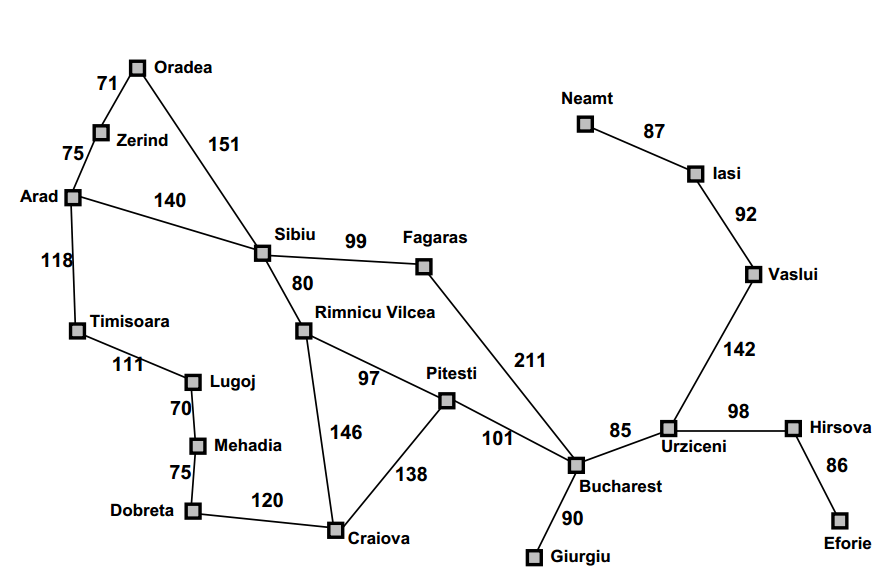
\includegraphics[width=14cm]{./Resources/p1.png}
		\caption{نقشه شهرهای رومانی}
	\end{figure}
	جزئیات فرموله‌کردن و مفروضات مورد استفاده در فرموله کردن این مسئله در بخش پیوست
	\ref{p1-app}
	قابل مشاهده است.\\
	\subsubsection{جستجوی سطح اول}
	آزمایش جستجوی سطح اول روی این مسئله با فرموله‌بندی موجود در پیوست
	\ref{p1-app}
	انجام شد و نتایج این آزمایش در جدول
	\ref{p1-bfs}
	قابل مشاهده است.
	\begin{table}[H]
		\centering
		\caption{نتایج جستجوی گراف شهرهای رومانی با استفاده از الگوریتم اول سطح.}
		\label{p1-bfs}
		\begin{tabular}{c|c}
			معیار                                   & نتیجه به دست آمده طی اجرای اگوریتم \\ \hline
			بهترین مسیر یافته شده &  \lr{Arad, Sibiu, Fagaras, Bucharest, Urziceni, Vaslui}\\
			هزینه مسیر یافته شده   &  ۶۷۷ واحد \\
			تعداد گره‌های بسط داده شده در حین جستجو & ۸۴ \\
			تعداد گره‌های مشاهده شده در حین جستجو   & ۳۳ \\
			حداکثر حافظه استفاده شده در حین جستجو   &  ۴۵                                 
		\end{tabular}
	\end{table}
	\subsubsection{جستجوی عمق اول با عمق محدود ۸}
	در پیاده‌سازی جستجوگر عمق اول در این فریم‌ورک، می‌بایست قبل از شروع جستجو مشخص شود که آیا جستجوی مورد نظر دارای عمق محدود است یا خیر. با ست کردن عمق ۸ برای این جستجوگر، نتایج آزمایش در جدول
	\ref{p1-dfs8}
	قابل مشاهده است.
	\begin{table}[H]
		\centering
		\caption{نتایج جستجوی گراف شهرهای رومانی با استفاده از الگوریتم اول عمق با عمق محدود ۸.}
		\label{p1-dfs8}
		\begin{tabular}{c|c}
			معیار                                   & نتیجه به دست آمده طی اجرای اگوریتم \\ \hline
			بهترین مسیر یافته شده &  \lr{Arad, Zerind, Oradea, Sibiu, Fagaras, Bucharest, Urziceni, Vaslui}\\
			هزینه مسیر یافته شده   &  ۸۳۴ واحد \\
			تعداد گره‌های بسط داده شده در حین جستجو & ۲۲ \\
			تعداد گره‌های مشاهده شده در حین جستجو   & ۱۴ \\
			حداکثر حافظه استفاده شده در حین جستجو   &  ۱۴                                 
		\end{tabular}
	\end{table}
	
	\subsubsection{جستجوی A*}
	در این جستجو، تابع شهودی مورد استفاده، فاصله واقعی هر شهر تا شهر مقصد بوده که از وب نتایج یافت شدند. جزئیات این تابع در پیوست
	\ref{p1-app}
	قابل مشاهده است. نتایج این آزمایش نیز در جدول
	\ref{p1-astar}
	ذکر شده است.
		\begin{table}[H]
		\centering
		\caption{نتایج جستجوی گراف شهرهای رومانی با استفاده از الگوریتم اول عمق با عمق محدود ۸.}
		\label{p1-astar}
		\begin{tabular}{c|c}
			معیار                                   & نتیجه به دست آمده طی اجرای اگوریتم \\ \hline
			بهترین مسیر یافته شده &  \lr{Arad, Sibiu, Fagaras, Bucharest, Urziceni, Vaslui}\\
			هزینه مسیر یافته شده   &  ۶۷۷ واحد \\
			تعداد گره‌های بسط داده شده در حین جستجو & ۳۲ \\
			تعداد گره‌های مشاهده شده در حین جستجو   & ۱۲ \\
			حداکثر حافظه استفاده شده در حین جستجو   &  ۲۴                                 
		\end{tabular}
	\end{table}
	\subsection{مسئله دوم: پازل ۸تایی}
	\subsubsection{جستجوی اول عمق گرافی}
	در جستجوی اول عمق گرافی نمونه داده شده در تعریف پروژه به مشکل عدم وجود حافظه کافی برخورد کردیم که با تغییر نمونه ورودی به ورودی زیر (فقط به عنوان تست) می‌توان پاسخ مناسب از آن گرفت:
	$1, 0, 2, 3, 4, 5, 6, 7, 8$
	\subsubsection{جستجوی دو جهته}
	با اجرای این الگوریتم با حالت اولیه ذکر شده در تعریف پروژه، که زمان بسیار زیادی برای اجرا نیاز داشت، به نتیجه‌ای نرسیدیم. اما با دادن حالت
	$ 1, 4, 2, 0, 3, 5, 6, 7, 8$
	به عنوان حالت اولیه، به نتایج ذکر شده در جدول
	\ref{p2-bds}
		رسیدیم.
		\begin{table}[H]
		\centering
		\caption{نتایج جستجوی دو جهته فضای حالت پازل ۸ تایی.}
		\label{p2-bds}
		\begin{tabular}{c|c}
			معیار                                   & نتیجه به دست آمده طی اجرای اگوریتم \\ \hline
			بهترین مسیر یافته شده &  \lr{012345678, 102345678, 142305678, 142035678}\\
			هزینه مسیر یافته شده   & ۳ \\
			تعداد گره‌های بسط داده شده در حین جستجو & ۹ \\
			تعداد گره‌های مشاهده شده در حین جستجو   & ۵ \\
			حداکثر حافظه استفاده شده در حین جستجو   & ۱۱                                 
		\end{tabular}
	\end{table}
	\subsubsection{جستجوی A* با تابع شهودی فاصله مستقیم}
	با اجرای الگوریتم داده شده و تابع شهودی مورد نظر، با حالت اولیه ذکر شده در قسمت قبل، در تعریف پروژه به نتایج ذکر شده در جدول
	\ref{p2-astar}
	رسیدیم.
		\begin{table}[H]
			\centering
			\caption{نتایج جستجوی دو جهته فضای حالت پازل ۸ تایی.}
			\label{p2-astar}
			\begin{tabular}{c|c}
				معیار                                   & نتیجه به دست آمده طی اجرای اگوریتم \\ \hline
				بهترین مسیر یافته شده &  \lr{012345678, 102345678, 142305678, 142035678}\\
				هزینه مسیر یافته شده   & ۳ \\
				تعداد گره‌های بسط داده شده در حین جستجو & ۱۲ \\
				تعداد گره‌های مشاهده شده در حین جستجو   & ۵ \\
				حداکثر حافظه استفاده شده در حین جستجو   & ۱۲                                 
			\end{tabular}
		\end{table}
	\subsection{مسئله سوم: مبلغین مذهبی و آدم‌خوارها}
	با پیاده‌‌سازی و فرموله‌بندی این سوال در متد
	\texttt{p3}
	فایل
	\texttt{Main.java}
	به اجرای الگوریتم‌های جستجوی مختلف روی این سوال پرداخته شد.
	\subsubsection{جستجوی سطح اول}
	نتایج جستجوی سطح اول در جدول
	\ref{p3-bfs}
	ذکر شده است.
			\begin{table}[H]
			\centering
			\caption{نتایج جستجوی سطح اول مسئله مبلغیم مذهبی و آدم‌خوارها}
			\label{p3-bfs}
			\begin{tabular}{c|c}
				معیار                                   & نتیجه به دست آمده طی اجرای اگوریتم \\ \hline
				بهترین مسیر یافته شده & (در سمت اولیه رود) ۳ آدم‌خوار و ۳ مبلغ، ۱ آدم‌خوار و ۳ مبلغ، ۱ آدم‌خوار و ۱ مبلغ، ۰ آدم‌خوار و ۰ مبلغ\\
				هزینه مسیر یافته شده   & ۳ \\
				تعداد گره‌های بسط داده شده در حین جستجو & ۳۲ \\
				تعداد گره‌های مشاهده شده در حین جستجو   & ۲۰ \\
				حداکثر حافظه استفاده شده در حین جستجو   & ۳۳                                 
			\end{tabular}
		\end{table}	 
	\subsubsection{جستجوی عمق اول با افزایش تدریجی عمق}
	نتایج جستجوی عمق اول با افزایش تدریجی عمق در جدول
	\ref{p3-dfs}
	قابل مشاهده است.
	\begin{table}[H]
		\centering
		\caption{نتایج جستجوی سطح اول مسئله مبلغیم مذهبی و آدم‌خوارها}
		\label{p3-dfs}
		\begin{tabular}{c|c}
			معیار                                   & نتیجه به دست آمده طی اجرای اگوریتم \\ \hline
			بهترین مسیر یافته شده & (در سمت اولیه رود) ۳ آدم‌خوار و ۳ مبلغ، ۱ آدم‌خوار و ۳ مبلغ، ۱ آدم‌خوار و ۱ مبلغ، ۰ آدم‌خوار و ۰ مبلغ\\
			هزینه مسیر یافته شده   & ۳ \\
			تعداد گره‌های بسط داده شده در حین جستجو & ۵۸ \\
			تعداد گره‌های مشاهده شده در حین جستجو   & ۶۱ \\
			حداکثر حافظه استفاده شده در حین جستجو   & ۲۸                                 
		\end{tabular}
	\end{table}	 
	
	

	%%%%%%%%%%%%%%%%%%%%%%%%%%%%%%%
	%%   Results			     %%
	%%%%%%%%%%%%%%%%%%%%%%%%%%%%%%%
	%\newpage
	%	\section{نتایج}
	%%%%%%%%%%%%%%%%%%%%%%%%%%%%%%%
	%%   Discussion			     %%
	%%%%%%%%%%%%%%%%%%%%%%%%%%%%%%%
	%\newpage
	%	\section{بحث}
	این بحث در مورد نتایج به دست آمده است.
	%%%%%%%%%%%%%%%%%%%%%%%%%%%%%%%
	%%   CONCLUSION			     %%
	%%%%%%%%%%%%%%%%%%%%%%%%%%%%%%%
	%\newpage
	%	\section{نتیجه گیری}
	این نتیجه گیری از بحث هاست.
	%%%%%%%%%%%%%%%%%%%%%%%%%%%%%%%
	%%   ACKNOWLEDGMENTS	     %%
	%%%%%%%%%%%%%%%%%%%%%%%%%%%%%%%
	%\newpage
	%\section*{تشکر و قدردانی}
	%%%%%%%%%%%%%%%%%%%%%%%%%%%%%%%
	%%   REFERENCES			     %%
	%%%%%%%%%%%%%%%%%%%%%%%%%%%%%%%
	%\newpage
	%\begin{thebibliography}{20}
	\begin{LTRitems}
	\end{LTRitems}
\end{thebibliography}
	%%%%%%%%%%%%%%%%%%%%%%%%%%%%%%%
	%%   Appendix			     %%
	%%%%%%%%%%%%%%%%%%%%%%%%%%%%%%%
	\newpage
	\appendix
\section{پیوست}
\subsection{مسئله اول: مسیریابی شهرهای رومانی} \label{p1-app}
هرکدام از شهرها به ترتیب ذکر شده در شکل
\ref{p1-edited}
شماره‌گذاری شدند. در تابع شهودی مورد استفاده، فاصله واقعی هرکدام از شهرها نسبت به مقصد داده شده مورد استفاده قرار می‌گرفت که به ترتیب ذکر شده عبارتند از (عدد نوشته شده در هر سطر بیانگر فاصله واقعی آن شهر -مقدار تابع شهودی- تا مقصد است.):
\begin{latin}
	\begin{lstlisting}
710,
634,
576,
677,
408,
636,
720,
669,
561,
507,
330,
447,
388,
324,
267,
283,
387,
0,
66.6,
133,
\end{lstlisting}
\end{latin}

\begin{figure}[H]
	\centering
	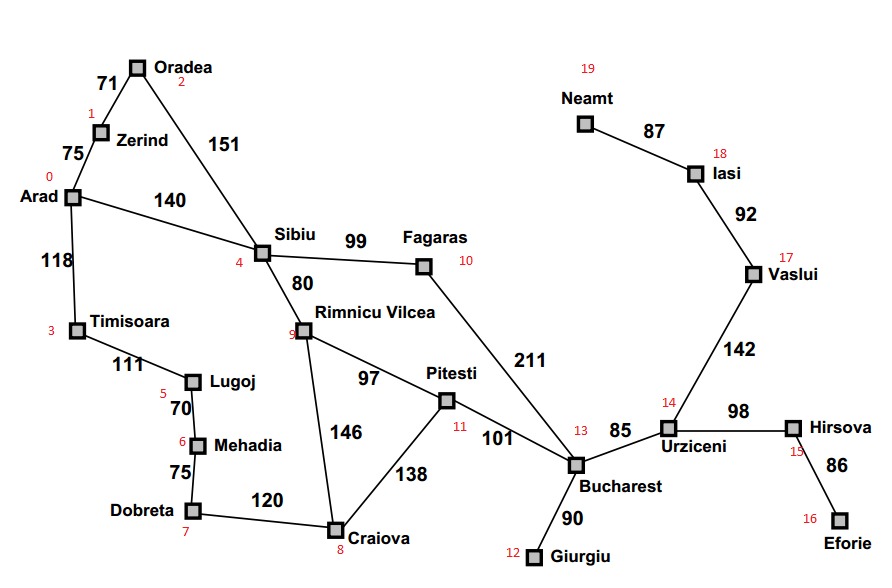
\includegraphics[width=14cm]{./Resources/p1e.png}
	\caption{شماره‌گذاری شهرهای رومانی.}
	\label{p1-edited}
\end{figure}
	\newpage
	
\end{document}